\scanpage{28}
\margin{27}

artificiels aux bord du disque, \unsure{sûrement rédhibitoires}, i.e. \unsure{certaines|certains} ps. droites de $\Delta(D)$, qui \unsure{se rencontraient} pas dans $\Delta(D)$, vont se rencontrer sur le bord de $\Delta'(D)$ \deleted{\unsure{;} }. Si on fait par contre les recollements \deleted{\unsure{sur}} \inserted{des} $\Delta(D)$, sans faire les identifications qui mènent aux $\Delta'(D)$, on trouve une \uline{surface à bord} (\inserted{bord} en vert), d'où à nouveau, en bouchant les trous \inserted{par des disques $\Delta_\alpha$}, une surface sans bord compacte. (On obtient la surface envisagée au début en contractant \inserted{chacun des} ces disques en \deleted{\unsure{des}} un point.) La surface cellulaire à bord obtenue est telle que les pts du bord sont \deleted{doubles ou triples} \inserted{tous d'ordre 2 ou trois}, et chaque sommet est sur le bord, elle se déduit de la carte sans bord par le procédé canonique, consistant à enlever un petit disque autour de chaque sommet. En tous cas, les trous à boucher dans la surface à bord correspondent exactement aux sommets de la surface sans bord.

\margin{\unsure{avec un grain de sel} $\nearrow$}

\uline{25.12}

Il faudrait regarder la \unsure{relation} entre $\operatorname{Pol}(D)$ et $\operatorname{Pol}(D')$, quand $D\longrightarrow D'$ et $D'$ supercritique. Il faudrait déjà \uline{définir} $\operatorname{Pol}(D')$, i.e. $\operatorname{Pol}(\Delta)$ quand $\Delta\in\Sigma$, comme l'une des \unsure{générisations} de $\Delta$, avec une structure polygonale convenable dessus. On a vu que les \deleted{\unsure{spécialisations}} \unsure{générisations} de $\Delta$ correspondent aux sommets sur $\widetilde\Delta$, image inverse de $\Delta$ dans $\widetilde X$. D'ailleurs pour un sommet $s$ de $\Delta$,

\figure{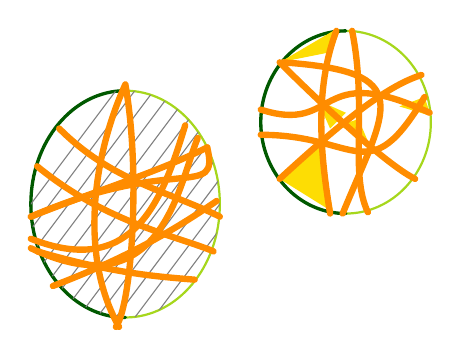
\begin{tikzpicture}[x=.8cm,y=.8cm,line cap=round,line join=round]
\begin{scope}[shift={(0,0)}]
\draw[yellow!65!green,thick] (0,0) ellipse(1.5 and 1.8);\draw[green!35!black,very thick] (90:1.5 and 1.8) arc(90:270:1.5 and 1.8);
\begin{scope}\clip (0,0) ellipse(1.5 and 1.8);\foreach \t in {-3,-2.7,...,2}{\draw[gray] (\t,-2)--({\t+3},2);}\end{scope}
\draw[orange!90!yellow,line width=2.3pt] (0,1.9)..controls(-.5,.8)and(-.75,-.8)..(-.1,-1.95) (0,1.9)..controls(.25,.5)and(.1,-1.6)..(-.15,-1.95);
\draw[orange!90!yellow,line width=2.3pt] (-1.05,1.2)..controls(-.2,.35)and(.7,.2)..(1.5,-.2) (-1.4,.6)..controls(-.3,-.3)and(.8,-.5)..(1.4,-.75);
\draw[orange!90!yellow,line width=2.3pt] (-1.5,-.2)..controls(-.5,.2)and(.5,.5)..(1.3,.9) (-1.5,-.55)..controls(.15,-1.2)and(.6,.1)..(.95,1.25);
\draw[orange!90!yellow,line width=2.3pt] (-1.5,-.7)..controls(.6,-1.7)and(.85,.35)..(1.15,1.05) (-1.15,-1.3)..controls(-.1,-.9)and(.65,-.5)..(1.45,.05);
\draw[orange!90!yellow,line width=2.3pt] (-1.4,-.75)..controls(-.2,-1.1)and(.5,-1.15)..(1.1,-1.2) (-1.5,-.2)..controls(.8,.8)and(1.5,.05)..(1.3,.9);
\end{scope}
\begin{scope}[shift={(3.5,1.3)}]
\draw[yellow!65!green,thick] (0,0) ellipse(1.35 and 1.45);\draw[green!35!black,very thick] (90:1.35 and 1.45) arc(90:270:1.35 and 1.45);
\fill[yellow!80!orange] (-1.05,.95)--(-.2,1.45)--(-.3,1.1)--cycle;
\fill[yellow!80!orange] (-1.05,-.9)--(-.42,-.3)--(-.2,-1.43)--cycle;
\fill[yellow!80!orange] (-.45,.35)--(-.25,-.1)--(0,.15)--cycle;
\fill[yellow!80!orange] (.2,.05)--(.35,-.3)--(-.1,-.05)--cycle;
\fill[yellow!80!orange] (1.25,.4)--(1.35,.1)--(.85,.25)--cycle;
\draw[orange!90!yellow,line width=2.3pt] (-.15,1.45)..controls(-.55,.4)and(-.35,-.8)..(-.25,-1.45) (.1,1.45)..controls(.35,.2)and(.05,-.8)..(.35,-1.43);
\draw[orange!90!yellow,line width=2.3pt] (-1.05,.95)..controls(-.2,.1)and(.7,-.7)..(1.1,-.9) (-1.35,.2)..controls(-.1,-.2)and(-.5,1)..(1.33,.15);
\draw[orange!90!yellow,line width=2.3pt] (-1.35,-.2)..controls(.2,-.2)and(.35,-1.1)..(1.25,.4) (-1.05,-.9)..controls(.2,.25)and(.75,.6)..(1.2,.75);
\draw[orange!90!yellow,line width=2.3pt] (-1,.95)..controls(1.15,.8)and(.65,.25)..(-.05,-1.45);
\end{scope}
\end{tikzpicture}}
